%%%%%%%%%%%%%%%%%%%%%%%%%%%%%%%%%%%%%%%%%
% a0poster Portrait Poster
% LaTeX Template
% Version 1.0 (22/06/13)
%
% The a0poster class was created by:
% Gerlinde Kettl and Matthias Weiser (tex@kettl.de)
% 
% This template has been downloaded from:
% http://www.LaTeXTemplates.com
%
% License:
% CC BY-NC-SA 3.0 (http://creativecommons.org/licenses/by-nc-sa/3.0/)
%
%%%%%%%%%%%%%%%%%%%%%%%%%%%%%%%%%%%%%%%%%

%----------------------------------------------------------------------------------------
%	PACKAGES AND OTHER DOCUMENT CONFIGURATIONS
%----------------------------------------------------------------------------------------

\documentclass[a0,portrait]{a0poster}

\usepackage{multicol} % This is so we can have multiple columns of text side-by-side
\columnsep=100pt % This is the amount of white space between the columns in the poster
\columnseprule=3pt % This is the thickness of the black line between the columns in the poster

\usepackage[svgnames]{xcolor} % Specify colors by their 'svgnames', for a full list of all colors available see here: http://www.latextemplates.com/svgnames-colors

\usepackage{times} % Use the times font
%\usepackage{palatino} % Uncomment to use the Palatino font

\usepackage{graphicx} % Required for including images
\graphicspath{{figures/}} % Location of the graphics files
\usepackage{booktabs} % Top and bottom rules for table
\usepackage[font=small,labelfont=bf]{caption} % Required for specifying captions to tables and figures
\usepackage{amsfonts, amsmath, amsthm, amssymb} % For math fonts, symbols and environments
\usepackage{wrapfig} % Allows wrapping text around tables and figures
\usepackage[utf8]{inputenc}
\usepackage{enumitem}
\usepackage{color}
\usepackage{tikz}
\usepackage{pgfplots}
\usepackage{colortbl, xcolor}
\usepackage{multicol}

\renewcommand\abstractname{\large Abstract}

%definicion para grafico en analisis de fold
\usetikzlibrary{shapes.geometric, arrows}

\tikzstyle{datos} = [rectangle, rounded corners, minimum width=12cm, minimum height=1cm,text centered, draw=black, fill=red!30]
\tikzstyle{train} = [rectangle, rounded corners, minimum width=2cm, minimum height=1cm,text centered, draw=black, fill=red!30]
\tikzstyle{test} = [rectangle, minimum width=2cm, minimum height=0.5cm, text centered, draw=black, fill=orange!30]
\tikzstyle{prom} = [rectangle, rounded corners, minimum width=8cm, minimum height=0.5cm, text centered, draw=black, fill=blue!30]
\tikzstyle{fold} = [rectangle, minimum width=2cm, minimum height=0.5cm, text centered]
\tikzstyle{proc} = [trapezium, trapezium left angle=70, trapezium right angle=110, minimum width=3cm, minimum height=0.8cm, text centered, text width=2.5cm, draw=black, fill=blue!30]

\tikzstyle{arrow} = [thick,->,>=stealth]
\tikzstyle{arrowBig} = [line width=8pt,->,>=stealth]

%fin fold

%definicion otros x validations
\usetikzlibrary{shapes.geometric}
\tikzset{myshade/.style={minimum size=.4cm,shading=radial,inner color=white,outer color={#1!90!gray}}}
\newcommand\mycirc[1][]{\tikz\node[circle,myshade=#1]{};}

\begin{document}

%----------------------------------------------------------------------------------------
%	POSTER HEADER 
%----------------------------------------------------------------------------------------

% The header is divided into two boxes:
% The first is 75% wide and houses the title, subtitle, names, university/organization and contact information
% The second is 25% wide and houses a logo for your university/organization or a photo of you
% The widths of these boxes can be easily edited to accommodate your content as you see fit

\begin{minipage}[b]{0.75\linewidth}
\veryHuge \color{NavyBlue} \textbf{Sistema de grabación para detectar hablantes de Buenos Aires y Córdoba} \color{Black}\\ % Title
%\Huge\textit{An Exploration of Complexity}\\[2cm] % Subtitle
\huge \textbf{Fernando Bugni, Agustín Gravano \& Miguel Martínez Soler}\\[0.5cm] % Author(s)
\huge Universidad de Buenos Aires - Facultad de Ciencias Exactas y Naturales\\[0.4cm] % University/organization
\Large \texttt{fernando.bugni@gmail.com, gravano@dc.uba.ar, miguelmsoler@gmail.com} \\
\end{minipage}
%
\begin{minipage}[b]{0.25\linewidth}

\includegraphics[width=12cm]{logo-uba.png}\\
\end{minipage}

\vspace{1cm} % A bit of extra whitespace between the header and poster content

%----------------------------------------------------------------------------------------

\begin{multicols}{2} % This is how many columns your poster will be broken into, a portrait poster is generally split into 2 columns

%----------------------------------------------------------------------------------------
%	ABSTRACT
%----------------------------------------------------------------------------------------

\color{Navy} % Navy color for the abstract

\begin{abstract}
	
\large El uso de la lengua siempre ha caracterizado a las personas que la utilizan. La forma como nos comunicamos no sólo posee la información del mensaje a transmitir, sino que también posee características del hablante. Nos enfocaremos en distinguir estas características entre las regiones de Córdoba y Buenos Aires. En el presente trabajo desarrollamos un sistema de grabación a través de Internet que nos permitió recolectar grabaciones de hablantes provenientes de ambos grupos. Diseñamos un experimento que nos ayudó a comparar el habla de cada grupo haciendo hincapié en sus diferencias. Extrayendo estos atributos, utilizamos algoritmos de Machine Learning para la clasificación de hablantes en los dos grupos.

\end{abstract}

%----------------------------------------------------------------------------------------
%	INTRODUCTION
%----------------------------------------------------------------------------------------

\color{SaddleBrown} % SaddleBrown color for the introduction

\section*{Introduction}

\large

%En la literatura existen estudios que explican diferencias entre ambos grupos, por ejemplo \textit{El español en la Argentina} \cite{Fontanella2000} de Beatriz Fontanella de Weinberg y \textit{Español en la Argentina} \cite{Vidal1964} de Elena Vidal de Battini. 

Las diferencias estudiadas entre los dos grupos son: 

\begin{itemize}
	
	\item \textbf{Regla 1: Los hablantes de Córdoba estiran la sílaba anterior a la acentuada mientras los de Buenos Aires no lo hacen.}  Ejemplo: `Espectacular' posee su sílaba acentuada en `-lar'. La sílaba anterior, o sea `-cu-' se alarga solamente para hablantes de Córdoba. 
	
	\item \textbf{Regla 2: Los hablantes de Córdoba aspiran y elisionan la /s/ al finalizar una palabra. Esto no sucede en Buenos Aires.} Ejemplo: `Pájaros' posee el fonema /s/ al final. Utilizando la dialéctica de Córdoba, la /s/ final sería más suave que una de Buenos Aires. 
	
	\item \textbf{Regla 3: Para hablantes de Córdoba, la /s/ antes de la /c/ o /t/ suenan más suaves que para hablantes de Buenos Aires.} Ejemplo: `Mosca' en la variante de Córdoba posee el fonema /s/ más suave que en Buenos Aires.
	
	\item \textbf{Regla 4: La `c' antes de la `t' se pronuncia con menor frecuencia para hablantes de Córdoba que para hablantes de Buenos Aires.} Ejemplo: `Doctor' no debe sonar el fonema /c/.
	
	\item \textbf{Regla 5: Para hablantes cordobeces la `y’ y `ll’ se pasa a `i’. No sucede esto para Buenos Aires.} Ejemplo: `lluvia' se debe pronunciar utilizando el fonema /j/. 
	
	\item \textbf{Regla 6: En hablantes cordobeces la /r/ no vibra mientras que en Buenos Aires pasa lo contrario.} Ejemplo: `Espárrago' en su fonema /r/ debe ser suave en comparación con Buenos Aires. 
	
\end{itemize}

Normalmente estas reglas se producen en el \textbf{habla espontánea} y raramente en habla leída. 

%----------------------------------------------------------------------------------------
%	OBJECTIVES
%----------------------------------------------------------------------------------------

\color{DarkSlateGray} % DarkSlateGray color for the rest of the content

\section*{Diseño del experimento}

Definimos dos tipos de frases para grabar durante el experimento: \textbf{Frases comunes} y \textbf{Frases Amper}. 

\begin{enumerate}
\item \textbf{Frases comunes}: 

	Agregamos 30 frases populares con el objetivo de captar pronunciación espontánea. Con ellas vamos a cubrir las reglas 2 a 6. Ejemplo: \textbf{`En la pelea se conoce al soldado,} \textbf{sólo en la \underline{victoria} se conoce al \underline{caballero}’}. \textbf{`victoria’} cubre la regla 4 que nos propone medir la duración de la \textit{/c/} antes de la \textit{/t/}. \textbf{`caballero’} para la regla 5: el fonema \textit{/ll/} se pasa a \textit{/i/} 
	
\item \textbf{Frases Amper}:
	
	Para captar sílabas acentuadas y su sílaba anterior a la acentuada se agregó frases con una estructura fija. El objetivo es cubrir la regla 1. \textbf{Esquema: \textit{Sujeto+`` \textbf{salió} ’’+Adjetivo}}. Donde \textbf{Sujeto}: \textit{``El canapé’’, ``El repollo’’, ``El espárrago’’}; \textbf{Adjetivo}: \textit{``espectacular’’, ``delicioso’’, ``riquísimo’’}. Todas las combinaciones agregan 9 frases más.

\end{enumerate}

\large \textbf{Combinamos las frases}: el orden de frases en una instancia del experimento va ser intercalado 1 ó 3 Frases comunes cada una Amper. Un ejemplo sería: 

	\begin{tikzpicture}[scale=3.5]
	%1-3 comun 4 amper 5-6 comun 6 amper 7-9 comun
	%10 amper 11-13 comun 14 amper
	%\fill[red!20](0,0) rectangle (0.4,0.4); 
	%\fill[blue!20!white](0.4,0) rectangle (0.8,0.4); 
	\fill[blue!20!white](0,0) rectangle (0.4*3,0.4);
	\fill[red!20](0.4*3,0) rectangle (0.4*5,0.4); 
	\fill[blue!20!white](0.4*5,0) rectangle (0.4*7,0.4);
	\fill[red!20](0.4*7,0) rectangle (0.4*8,0.4); 
	\fill[blue!20!white](0.4*8,0) rectangle (0.4*10,0.4);
	\fill[red!20](0.4*10,0) rectangle (0.4*11,0.4);
	\fill[blue!20!white](0.4*11,0) rectangle (0.4*13,0.4);
	\fill[red!20](0.4*13,0) rectangle (0.4*14,0.4);
	\fill[blue!20!white](0.4*14,0) rectangle (0.4*16,0.4);
	\fill[red!20](0.4*16,0) rectangle (0.4*17,0.4);			
	\fill[blue!20!white](0.4*17,0) rectangle (0.4*19,0.4);
	\fill[red!20](0.4*19,0) rectangle (0.4*20,0.4);			
	\fill[blue!20!white](0.4*20,0) rectangle (0.4*22,0.4);
	\fill[red!20](0.4*22,0) rectangle (0.4*24,0.4);			
	\fill[blue!20!white](0.4*24,0) rectangle (0.4*25,0.4);
	
	\draw[step=0.4cm,very thin,fill=blue!20!white] (0,0) grid (10,0.4);
	
	\end{tikzpicture}
	
	\begin{multicols}{2}
		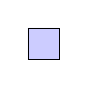
\begin{tikzpicture}
		\draw[step=0.4cm,very thin,fill=blue!20!white] (0,0) grid (0.4,0.4) rectangle (0,0);
		\end{tikzpicture} Frases comúnes
		
		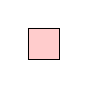
\begin{tikzpicture}
		\draw[step=0.4cm,very thin,fill=red!20] (0,0) grid (0.4,0.4) rectangle (0,0);
		\end{tikzpicture} Frases Amper
	\end{multicols}	

%----------------------------------------------------------------------------------------
%	MATERIALS AND METHODS
%----------------------------------------------------------------------------------------

\section*{Datos Obtenidos}

\begin{wraptable}{l}{18cm}
	\begin{tabular}{l c c c c}
		\toprule
		\textbf{}  & \textbf{Bs.As. } & \textbf{Cba.} & \textbf{Total} \\ 
		\midrule
		%\textbf{Conservar}  & 222 & 105 & 327 \\ \hline
		\textbf{Conservar}  & 220 & 90 & 310 \\ 
		\textbf{Problemas en el habla}  & 33 & 15 & 48 \\ 
		\textbf{Mucho ruido de fondo}  & 2 & 12 & 14 \\ 
		\textbf{Sonido saturado}  & 2 & 0 & 2 \\ 
		\bottomrule
	\end{tabular}
	\captionof{table}{Grabaciones y su clasificación}
\end{wraptable}

\large Utilizando nuestra página web del experimento categorizamos las grabaciones recolectadas en la \textbf{tabla 1}. La página de grabación también soporta varios intentos para una misma grabación. Descartamos estos casas quedándonos con el mejor caso.
Esto nos da un total de \textbf{260 grabaciones, 181 para Buenos Aires y 79 para Córdoba.} Seguiremos con estos datos para el posterior análisis.

%------------------------------------------------

\section*{Extracción de información}

\large 
Etiquetamos cada audio para marcar dónde comienza y termina cada fonema. Para ello utilizamos una librería llamada \textbf{ProsodyLab-Aligner}. Un ejemplo extrayendo el atributo 'kt' es el siguiente:

\begin{center}
	{\textbf{\textit{``en la pelea se konose al soldaDo \\solo en la biktorja se konose al kaBaZero’’}}}
\end{center}

\begin{center}
	\begin{tikzpicture}[xscale=2]
	\draw[x=2cm,step=0.05pt,thick,>=latex](0,0) -- (7.5,0);
	\foreach \Xc in {0,...,15}
	{
		\draw[thick] 
		(\Xc,0) -- ++(0,05pt);
	}
	\draw[dotted,thick] (-0.5,0) -- (0,0);
	\draw[dotted,thick] (15,0) -- (15.5,0);
	% la victoria se conoce
	\foreach \Xc/\Texto in 
	{5/k}
	{
		\fill[black] 
		([xshift=2pt]\Xc,0.05)  
		rectangle node[above] {\strut\large\Texto} 
		([xshift=-2pt]\Xc+1,0.15);  
	}
	\foreach \Xc/\Texto in 
	{0/l,1/a,2/$sil$,3/b,4/i,6/t,7/o,8/r,9/j,10/a,11/$sil$,12/s, 13/e, 14/$sil$}
	{
		\node[above] at ([xshift=15pt]\Xc,0.05){\strut\large\Texto} ;
	}
	\end{tikzpicture}
\end{center}

\large {
La métrica utilizada es: \textbf{$\frac{ X - \mu }{ \sigma }$} donde $X$ es el valor a normalizar (por ej.: la duración de un fonema o sílaba dado). $\mu$ es el promedio de duración de la unidad utilizada en la grabación. $\sigma$ es el desvío estándar de esta unidad utilizada. Esta métrica la realizamos para cada una de las reglas.
}

\section*{Análisis de datos y clasificación}

Realizamos tres tipos de cross-validations para realizar la clasificación. 

\begin{itemize}
	\item \textbf{CV1 - Grupos de hablantes:} dividimos los hablantes en dos grupos en train y test. Esto lo hacemos para 5 folds.\\
			\begin{center}
				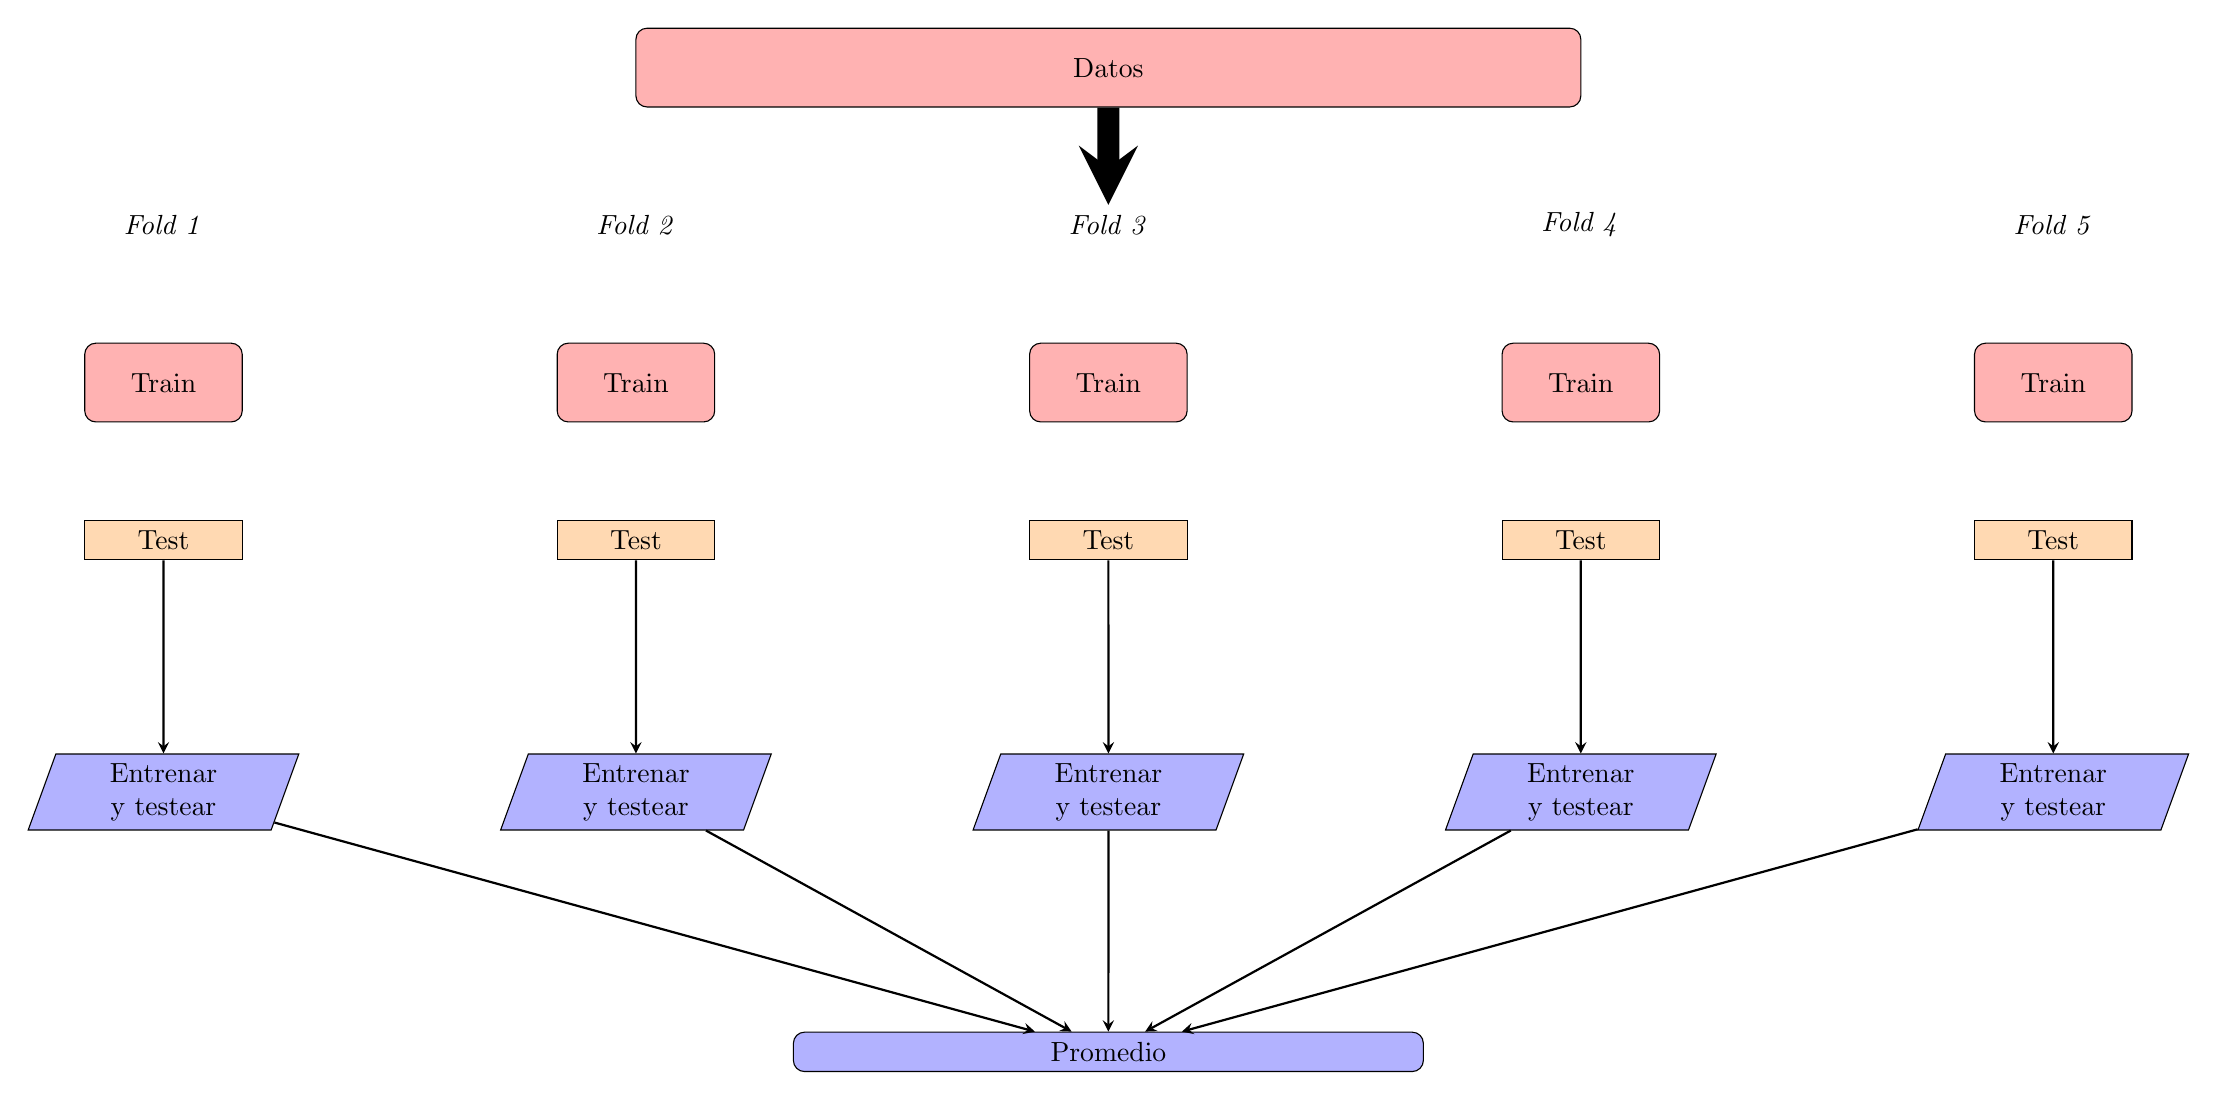
\begin{tikzpicture}[node distance=2cm, scale=1, every node/.style={scale=1}]
		
		\node (train1) [train] {Train};
		\node (train2) [train, xshift=-6.0cm] {Train};
		\node (train3) [train, xshift=-12.0cm] {Train};
		\node (train4) [train, xshift=-18.0cm] {Train};
		\node (train5) [train, xshift=-24.0cm] {Train};
		
		\node (data) [datos, below of=train5, yshift=6.0cm,  xshift=12.0cm] {Datos};
		
		\node (fold1) [fold, above of=train5] {\textit{Fold 1}};
		\node (fold2) [fold, above of=train4] {\textit{Fold 2}};
		\node (fold3) [fold, above of=train3] {\textit{Fold 3}};
		\node (fold4) [fold, above of=train2] {\textit{Fold 4}};
		\node (fold5) [fold, above of=train1] {\textit{Fold 5}};
		
		\node (test1) [test, below of=train1] {Test};
		\node (test2) [test, below of=train2] {Test};
		\node (test3) [test, below of=train3] {Test};
		\node (test4) [test, below of=train4] {Test};
		\node (test5) [test, below of=train5] {Test};
		
		\node (proc1) [proc, below of=test1, yshift=-1.2cm] {Entrenar y testear};
		\node (proc2) [proc, below of=test2, yshift=-1.2cm] {Entrenar y testear};
		\node (proc3) [proc, below of=test3, yshift=-1.2cm] {Entrenar y testear};
		\node (proc4) [proc, below of=test4, yshift=-1.2cm] {Entrenar y testear};
		\node (proc5) [proc, below of=test5, yshift=-1.2cm] {Entrenar y testear};
		
		\node (prom) [prom, below of=test3, yshift=-4.5cm] {Promedio};
		
		\draw [arrowBig] (data) -- (fold3);
		
		\draw [arrow] (test1) -- (proc1);
		\draw [arrow] (test2) -- (proc2);
		\draw [arrow] (test3) -- (proc3);
		\draw [arrow] (test4) -- (proc4);
		\draw [arrow] (test5) -- (proc5);
		
		\draw [arrow] (proc1) -- (prom);
		\draw [arrow] (proc2) -- (prom);
		\draw [arrow] (proc3) -- (prom);
		\draw [arrow] (proc4) -- (prom);
		\draw [arrow] (proc5) -- (prom);
		
		\end{tikzpicture}
			\end{center}
	
	\item \textbf{CV2 - Dejando un hablante fuera promediando los atributos: } En este esquema dejamos un hablante afuera para test y entrenamos con el resto. También equilibramos la cantidad de hablantes: 8 Buenos Aires, 8 Córdoba. Para cada hablante promediamos sus atributos.
	
	\begin{center}
		\mycirc[blue] Hablante para train \mycirc[red] Hablante para test

		\begin{tabular}{cccccccccccc}
			& \multicolumn{11}{c}{\textit{Número de hablante}} \\
			& 1 & 2 & 3 & 4 & 5 & 6 & 7 & ... & 14 & 15 & 16 \\
			\hline \\
			Fold 1 &\mycirc[red] & \mycirc[blue] & \mycirc[blue]  & \mycirc[blue]  & \mycirc[blue]  & \mycirc[blue]  & \mycirc[blue] & ... & \mycirc[blue] & \mycirc[blue] & \mycirc[blue]  \\
			
			Fold 2 &\mycirc[blue] & \mycirc[red] & \mycirc[blue]  & \mycirc[blue]  & \mycirc[blue]  & \mycirc[blue]  & \mycirc[blue] & ... & \mycirc[blue] & \mycirc[blue] & \mycirc[blue]  \\
			
			Fold 3 &\mycirc[blue] & \mycirc[blue] & \mycirc[red]  & \mycirc[blue]  & \mycirc[blue]  & \mycirc[blue]  & \mycirc[blue] & ... & \mycirc[blue] & \mycirc[blue] & \mycirc[blue]  \\
			
			\multicolumn{11}{c}{\textit{...}}	\\
			
			Fold 16 &\mycirc[blue] & \mycirc[blue] & \mycirc[blue]  & \mycirc[blue]  & \mycirc[blue]  & \mycirc[blue]  & \mycirc[blue] & ... & \mycirc[blue] & \mycirc[blue] & \mycirc[red]   \\
			
		\end{tabular}
	\end{center}
	
	\item \textbf{CV3 - Dejando un hablante fuera promediando los atributos desconocidos}: No es necesario promediar todos los atributos de cada hablante. Podemos promediar sólo los atributos desconocidos. El esquema de folds es igual al anterior.
	
\end{itemize}

\section*{Resultados}

En la \textbf{tabla 2} podemos ver el resultado del promedio de cada fold según cada clasificador.

\begin{wraptable}{l}{22cm}
	\begin{tabular}{l c c c c c c }
		\toprule
		\textbf{}  & \textbf{Zero Rule} & \textbf{Ripper} & \textbf{C4.5} & \textbf{F. SMO} & \textbf{NaiveBayes} \\ 
		\midrule
		\textbf{CV1} & 64 & 61 & 60 & 72 & 70 \\ 
		\textbf{CV2} & 53.33 & 60 & 60 & 93.33 & 80  \\
		\textbf{CV3} & 50 & 72.44 & 73.48 & 77.19 & 74.62 \\ 
		\bottomrule
	\end{tabular}
	\captionof{table}{Porcentaje de clasificación}
\end{wraptable}

Podemos ver cómo \textbf{Function SMO} y \textbf{NaiveBayes} pudieron mejorar la performance de clasificación utilizando los atributos que definimos. Utilizando Wilcoxon y T de Student pudimos confirmar que estos porcentajes son estadísticamente significativos. 

%----------------------------------------------------------------------------------------
%	REFERENCES
%----------------------------------------------------------------------------------------
{\small 
\nocite{*} % Print all references regardless of whether they were cited in the poster or not
\bibliographystyle{plain} % Plain referencing style
\bibliography{sample} % Use the example bibliography file sample.bib
}
\end{multicols}
\end{document}